\documentclass[11pt,a4paper]{article}
\usepackage[margin=2.5cm]{geometry}
\usepackage{amsmath, amssymb}
\usepackage{graphicx}
\usepackage{siunitx}
\usepackage{textcomp}
\usepackage{hyperref}

\title{01\_Data\_Preparation: MF4 $\rightarrow$ Cleaned 10\,ms Dataset}
\author{Validation\_Aero\_Test}
\date{\today}

\begin{document}
\maketitle

\section{Overview}
This document describes the data-preparation pipeline that converts raw telemetry
logs into a single analysis-ready CSV for downstream run extraction and drag
calculation.

\paragraph{Goal}
Produce a fixed-sample-rate dataset (\SI{10}{ms}) with stable, documented column
names.

\paragraph{Primary outputs}
\begin{itemize}
  \item Per-channel exports: \texttt{Outputs/01\_Data\_Preparation/Signals/*.csv}
  \item Canonical cleaned dataset: \texttt{Outputs/01\_Data\_Preparation/Aero\_Validation\_Signals\_cleaned\_10ms.csv}
\end{itemize}

\paragraph{Pipeline flow}
\begin{center}
\begin{verbatim}
Stint*.mf4
    |
    v
export_channels_10ms_to_signals.py    -->  Signals/<channel>.csv  (x N channels)
    |
    v
build_cleaned_signals_10ms.py         -->  Aero_Validation_Signals_cleaned_10ms.csv
    |
    v
load_data()  -->  sanitize_columns()  -->  add_derived_signals()
    |
    v
downstream (run extraction, drag calculation)
\end{verbatim}
\end{center}

\section{Inputs}
\begin{itemize}
  \item Raw logging data: \texttt{Data/<session>/Stint*.mf4}
  \item Channel list: \texttt{Data/channels\_extraction.txt} (one channel name per
        line; \texttt{\#} for comments)
\end{itemize}

% ---------------------------------------------------------------------------
\section{Step 1: Export per-channel CSVs}
% ---------------------------------------------------------------------------
Implemented in \texttt{Code/01\_Data\_Preparation/export\_channels\_10ms\_to\_signals.py}.

\subsection*{Concatenation strategy}
Each \texttt{Stint*.mf4} is treated as a separate segment:
\begin{itemize}
  \item Timestamps are shifted to start at 0 within the stint.
  \item Signals are interpolated onto a uniform grid with spacing $\Delta t$
        (default: \SI{0.01}{s}).
  \item Stints are concatenated on a continuous time axis with an optional
        single-$\Delta t$ gap between stints (enabled by default).
\end{itemize}

\subsection*{Per-channel output schema}
For each requested channel $c$, the exporter writes:
\begin{itemize}
  \item File: \texttt{Outputs/01\_Data\_Preparation/Signals/<channel>.csv}
  \item Columns: \texttt{time} (seconds) and \texttt{<channel\_name>} (numeric;
        NaN outside signal support).
\end{itemize}

% ---------------------------------------------------------------------------
\section{Step 2: Combine to the canonical cleaned dataset}
% ---------------------------------------------------------------------------
Implemented in \texttt{Code/01\_Data\_Preparation/build\_cleaned\_signals\_10ms.py}.

\subsection*{Join semantics}
All per-channel CSVs are read and joined on the time column using an outer join.
The resulting table is sorted by time; the index is reset and stored as column
\texttt{t\_s} (seconds).

\subsection*{Column sanitization}
Raw MF4 channel names contain brackets, units, and occasional encoding artifacts
(e.g., the degree symbol \texttt{\textdegree} may appear as a replacement
character). The function \texttt{aero\_validation.signals.sanitize\_columns}
(called automatically by \texttt{load\_data}) performs three operations:
\begin{enumerate}
  \item Strips leading/trailing whitespace from all column headers.
  \item Replaces mis-encoded characters with the correct symbol
        (e.g., replacement character $\rightarrow$ \texttt{\textdegree}).
  \item Maps known raw headers to canonical names via a static lookup table
        (defined in \texttt{\_column\_mapping}).  For example:
        \begin{center}
        \begin{tabular}{ll}
          \texttt{ICU\_Speedfl[km/h]}       & $\rightarrow$ \; \texttt{ICU\_Speedfl\_kmh} \\
          \texttt{SBG\_IMU\_ACCEL\_X[m.s-2]} & $\rightarrow$ \; \texttt{IMU\_ACCEL\_X\_ms2} \\
          \texttt{ICU\_SteeringAngle[\textdegree]} & $\rightarrow$ \; \texttt{ICU\_SteeringAngle\_deg} \\
        \end{tabular}
        \end{center}
  \item Drops unnamed trailing columns (e.g., empty columns from the logger).
\end{enumerate}
All downstream code works exclusively with the sanitized canonical names.

\subsection*{Canonical column naming}
The mapping in \texttt{\_column\_mapping} is the single source of truth for
channel naming.  If a new channel is added to the car, its raw header must be
added to this mapping so that downstream scripts see a stable name.  Names
follow the convention \texttt{<Source>\_<Signal>\_<Unit>}
(e.g., \texttt{GPS1\_VEL\_D\_ms}).

% ---------------------------------------------------------------------------
\section{Reproducibility}
% ---------------------------------------------------------------------------
The following commands reproduce the full data-preparation pipeline from raw
MF4 files (run from the repository root):

\begin{verbatim}
# Step 1: Export selected channels to per-channel CSVs at 10 ms
python Code/01_Data_Preparation/export_channels_10ms_to_signals.py \
    --stints-dir Data/<session> \
    --channels-file Data/channels_extraction.txt \
    --out-dir Outputs/01_Data_Preparation/Signals \
    --dt-ms 10

# Step 2: Combine per-channel exports into the canonical cleaned dataset
python Code/01_Data_Preparation/build_cleaned_signals_10ms.py \
    --channels-dir Outputs/01_Data_Preparation/Signals \
    --output Outputs/01_Data_Preparation/Aero_Validation_Signals_cleaned_10ms.csv
\end{verbatim}

% ---------------------------------------------------------------------------
\section{Derived signals}
% ---------------------------------------------------------------------------
All derived signals are computed by the public wrapper
\texttt{aero\_validation.signals.add\_derived\_signals}, which delegates to the
private sub-functions described below.  Each sub-function modifies the DataFrame
in place and can be tested independently.

% ---------------------------------------------------------------------------
\subsection{Notation}
% ---------------------------------------------------------------------------
The following time-synchronized columns are assumed to exist after sanitization:
\begin{itemize}
  \item $t$ [s]: timestamp \texttt{t\_s}.
  \item $\mathbf{a}_\text{IMU} = (a_x, a_y, a_z)$ [m/s$^2$]: IMU accelerations
        \texttt{IMU\_ACCEL\_X\_ms2}, \texttt{IMU\_ACCEL\_Y\_ms2},
        \texttt{IMU\_ACCEL\_Z\_ms2}.
  \item $v_\text{gps}$ [m/s]: GPS speed magnitude \texttt{GPS1\_VEL\_MAG\_ms}.
  \item $v_\text{wheel}$ [m/s]: wheel-speed magnitude, converted from
        \texttt{WHEEL\_SPEED\_kmh} by
        $v_\text{wheel} = \text{km/h} \cdot \frac{1000}{3600}$.
  \item $\theta$ [deg]: steering angle \texttt{ICU\_SteeringAngle\_deg}.
\end{itemize}

% ---------------------------------------------------------------------------
\subsection{Wheel speed}
% ---------------------------------------------------------------------------
\texttt{\_add\_wheel\_speed} computes \texttt{WHEEL\_SPEED\_kmh} as the
row-wise mean of the four available wheel-speed channels
(\texttt{ICU\_Speedfl\_kmh}, \texttt{ICU\_Speedfr\_kmh},
\texttt{ICU\_Speedrl\_kmh}, \texttt{ICU\_Speedrr\_kmh}).  If some channels are
missing, the mean is taken over the available subset.

% ---------------------------------------------------------------------------
\subsection{GPS speed magnitude}
% ---------------------------------------------------------------------------
\texttt{\_add\_gps\_speed\_magnitude} computes \texttt{GPS1\_VEL\_MAG\_ms}
from the three GPS velocity components when all are present:
\[
  v_\text{gps} = \sqrt{ v_D^2 + v_E^2 + v_N^2 }.
\]

% ---------------------------------------------------------------------------
\subsection{Zero-velocity mask}
% ---------------------------------------------------------------------------
\texttt{\_build\_zero\_velocity\_mask} identifies samples where the vehicle is
likely stationary.  Two speed sources are combined with a strict threshold of
\SI{0.05}{m/s}:
\[
  \mathcal{Z} = \{\, i \mid v_\text{gps}[i] < 0.05 \,\}
\]
If wheel speed is also available, the mask is tightened to the conjunction:
\[
  \mathcal{Z} = \{\, i \mid v_\text{gps}[i] < 0.05 \;\land\; v_\text{wheel}[i] < 0.05 \,\}.
\]

% ---------------------------------------------------------------------------
\subsection{IMU bias removal}
% ---------------------------------------------------------------------------
Inside \texttt{\_add\_imu\_longitudinal\_accel}, per-axis stationary biases are
estimated as medians over the zero-velocity mask $\mathcal{Z}$:
\[
  b_x = \operatorname{median}\{\, a_x[i] : i \in \mathcal{Z} \,\},
  \qquad b_y, b_z \text{ similarly}.
\]
If $|\mathcal{Z}| < 20$ samples, the global median of each axis is used as a
fallback.  Bias-corrected accelerations are then
\[
  a_x' = a_x - b_x,\quad a_y' = a_y - b_y,\quad a_z' = a_z - b_z.
\]

% ---------------------------------------------------------------------------
\subsection{Smoothing and $dv/dt$}
% ---------------------------------------------------------------------------
To obtain a stable numerical derivative of speed:
\begin{enumerate}
  \item Compute the median sample period $\Delta t_\text{med}$ from $t$ and set
        a smoothing window of approximately \SI{0.5}{s}
        ($\approx \frac{0.5}{\Delta t_\text{med}}$ samples, centered rolling
        mean).
  \item Smooth the speed trace (prefer $v_\text{gps}$, fall back to
        $v_\text{wheel}$) to obtain $\tilde{v}(t)$.
  \item Compute the numerical derivative:
        \[
          \frac{dv}{dt}(t) \approx \operatorname{gradient}\big(\tilde{v}(t),\,t\big).
        \]
\end{enumerate}

\paragraph{Speed source preference.}
GPS speed is preferred because it measures ground-referenced velocity with low
drift and is unaffected by tyre slip.  Wheel speed is always available (no
satellite dropouts) but can over- or under-report true speed during wheelspin or
lockup.  The fallback order ensures $dv/dt$ is computed whenever at least one
source is present.

% ---------------------------------------------------------------------------
\subsection{Straight and moving segment masking}
% ---------------------------------------------------------------------------
The axis-alignment weights (Section~6.8) are only fitted on samples where the
vehicle is moving and approximately straight, to avoid lateral-acceleration
contamination:
\begin{itemize}
  \item Moving mask: $\tilde{v}(t) > \SI{0.5}{m/s}$.
  \item Straight mask: $|\theta(t)| \le 5^\circ$ (if steering is available;
        otherwise skipped).
\end{itemize}
Samples must also have finite values in all required columns.

% ---------------------------------------------------------------------------
\subsection{Longitudinal axis estimation (least-squares)}
% ---------------------------------------------------------------------------
\texttt{\_fit\_accel\_alignment\_weights} estimates the longitudinal direction
in the IMU frame by regressing bias-corrected IMU signals onto $dv/dt$:
\begin{align*}
  A &= \begin{bmatrix} a_x' & a_y' & a_z' \end{bmatrix} \in \mathbb{R}^{N\times 3}, \\
  y &= \frac{dv}{dt} \in \mathbb{R}^{N}, \\[4pt]
  \mathbf{w} &= \arg\min_{\mathbf{w}\in\mathbb{R}^3} \| A\mathbf{w} - y \|_2^2.
\end{align*}
If fewer than 50 valid samples remain after masking, the fit falls back to the
identity assumption $\mathbf{w} = (1, 0, 0)$ (pure X-axis).

The longitudinal acceleration signal is then
\[
  a_\text{long}(t) = w_x\,a_x'(t) + w_y\,a_y'(t) + w_z\,a_z'(t),
\]
stored as column \texttt{IMU\_ACCEL\_LONG\_ms2}.

% ---------------------------------------------------------------------------
\section{Notes}
% ---------------------------------------------------------------------------
\begin{itemize}
  \item \textbf{Resampling}: interpolation is performed independently per
        channel; NaN indicates missing data or out-of-range timestamps.
  \item \textbf{Bias removal}: the ``stationary'' mask uses a strict low-speed
        threshold ($<\SI{0.05}{m/s}$) and falls back to global medians if too
        few stationary samples exist.
  \item \textbf{Longitudinal axis fit}: the least-squares weights are estimated
        only on straight + moving segments to avoid lateral acceleration
        contamination.  If fewer than 50 valid samples remain after masking,
        the fit falls back to $\mathbf{w} = (1, 0, 0)$ (pure X-axis).
  \item \textbf{Missing channels}: if a requested channel is absent from the
        MF4 file, the pipeline produces a NaN-filled column rather than
        crashing.  If multiple stints have different channel sets, the outer
        join fills missing segments with NaN.
  \item \textbf{GPS dropout}: the zero-velocity mask and $dv/dt$ computation
        fall back to wheel speed when GPS is unavailable, ensuring the pipeline
        degrades gracefully rather than failing.
  \item \textbf{Column mapping maintenance}: when the logger configuration
        changes, update \texttt{\_column\_mapping} in
        \texttt{aero\_validation/signals.py} to keep downstream code stable.
\end{itemize}

% ---------------------------------------------------------------------------
\section{Example outputs}
% ---------------------------------------------------------------------------
The figures below are diagnostic plots generated from the canonical cleaned
dataset.  They are produced by running the full data-preparation pipeline and
then plotting selected time windows (these specific plots are generated ad-hoc
and placed in \texttt{Outputs/01\_Data\_Preparation/plots/}).

The data shown is from the Stei\ss{}lingen aero-validation test day
(2025-10-22), comprising 4 stints and yielding approximately 46 coastdown runs
after extraction.

\begin{figure}[ht]
  \centering
  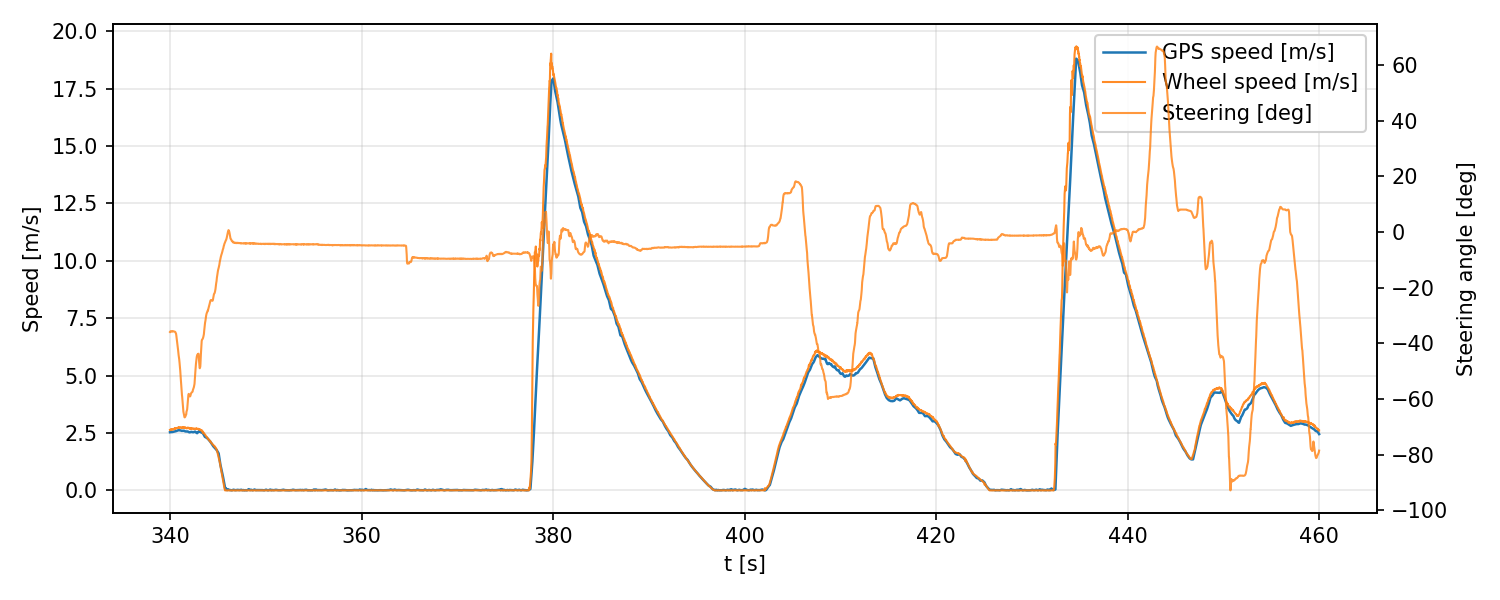
\includegraphics[width=\linewidth]{../../Outputs/01_Data_Preparation/plots/cleaned_speed_steering_example.png}
  \caption{Example time window showing GPS speed, wheel speed (converted to
           m/s), and steering angle from the cleaned dataset.}
\end{figure}

\begin{figure}[ht]
  \centering
  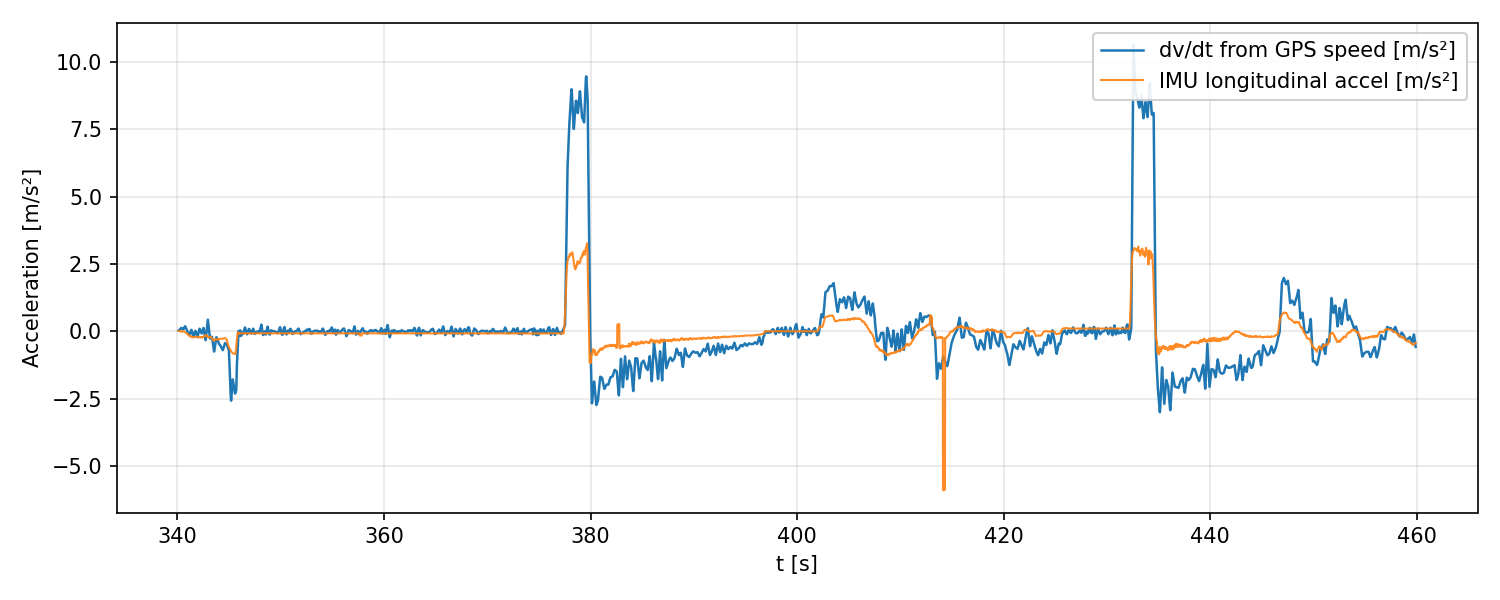
\includegraphics[width=\linewidth]{../../Outputs/01_Data_Preparation/plots/dvdt_vs_imu_long_example.png}
  \caption{Comparison between $dv/dt$ (computed from GPS speed) and the derived
           longitudinal IMU acceleration signal
           \texttt{IMU\_ACCEL\_LONG\_ms2}.}
\end{figure}

% ---------------------------------------------------------------------------
\section{Implementation references}
% ---------------------------------------------------------------------------
\begin{itemize}
  \item MF4 export:
        \texttt{Code/01\_Data\_Preparation/export\_channels\_10ms\_to\_signals.py}
  \item Combine \& derived signals:
        \texttt{Code/01\_Data\_Preparation/build\_cleaned\_signals\_10ms.py}
  \item Column sanitization \& mapping:
        \texttt{aero\_validation/signals.py} \; -- \;
        \texttt{sanitize\_columns}, \texttt{\_column\_mapping}
  \item Derived signals (public wrapper):
        \texttt{aero\_validation/signals.py} \; -- \;
        \texttt{add\_derived\_signals}
  \item Sub-functions (individually testable):
        \begin{itemize}
          \item \texttt{\_add\_wheel\_speed}
          \item \texttt{\_add\_gps\_speed\_magnitude}
          \item \texttt{\_build\_zero\_velocity\_mask}
          \item \texttt{\_add\_imu\_longitudinal\_accel}
          \item \texttt{\_fit\_accel\_alignment\_weights}
        \end{itemize}
  \item Data loading \& path resolution:
        \texttt{aero\_validation/io.py} \; -- \;
        \texttt{load\_data}, \texttt{data\_path}, \texttt{repo\_root}
\end{itemize}

The cleaned dataset produced by this pipeline is the input for the run
extraction step (see \texttt{02\_Run\_Extraction.pdf}) and ultimately for the
drag coefficient estimation (see \texttt{03\_Drag\_Calculation.pdf}).

\end{document}
